\chapter{Conclusion}
\label{chapter:conclusion}

This is the conclusion.  ce ați obținut, ce obiective ați avut, cum este relevant proiectul, ce rezultate ați obținut, cum ați evaluat.

Dynamic applications such as social networks generate large amounts of text data and the need for an application capable of clustering and aggregating all the content is increasing. Important issues such applications have to solve are both related to both semantics, short messages force an ambiguous text that needs to be decoded, and syntactical due to the fact that the same length constrains or due to the nature of the medium used to communicate.  
The Internet allows anyone to create content, publish and spread information. Social platforms are lowering the barrier of entry and are making it especially easy for everyone to have a voice on the Internet and as a result millions of messages and content of all forms is generated daily. Making sense of everything, and keeping track is becoming difficult and therefore it is time for tools that help understand the content to evolve and adapt to these mediums and make content exploration as easy as it is to post a message.
\newline
{\project}  attempts to solve this problem of content discovery and exploration. {\project}  endeavors to understand the topics being published and presents it to the user in a way that is accessible and easy to use. It creates clusters of messages by interpreting content and presents it to the user in a web interface that allows for him to browse through a large number of messages efficiently.
\newline
The feature that makes {\project}  relevant for the fast passed rate of tweets is its ability to parse the messages in real time. The data is not based on an archived corpus of documents but on streaming tweets as they happen. This way popular events, news and messages get reported in the interface and the user is able to keep in touch with what is happening right now.
\newline
\begin{itemize}
	\item Getting real time data from Twitter using its API based on user queries.
	\item Parsing tweets as they arrive. Using part-of-speech tagging to make annotations that help filter messages and extract important information.
	\item Using a clustering algorithm that is able to group messages, that has the ability to configure precision and that can run in parallel for a choice between speed and precision. 
	\item Building a decoupled system that can easily scale through the use of queues which allow for different rates of consumption and multiple consumers that can process the workload in parallel.
	\item Presenting the information through an accessible medium: the web browser, with an easy to use interface that allows the information to be explored.
\end{itemize}
Evaluating the results was done through the use of the frontend {\frontend}. We expanded the clusters and started exploring the different topics. \todo{more info}
One unexpected answer we got by running the application was discovering topic influencers. What we refer to as influencers are people with large following in social media that also are really engaged with their followers through comments, retweets and favorites. The way it comes up in {\project}  is that a lot of people will end up retweeting a certain tweet written by one of these accounts, and it will show up as a cluster composed of the same tweet. There is also an exception, meaning that cluster can be composed of a single tweet of an account with few followers if their message was in turn retweeted by an influencer. In this case the cluster is formed entirely out of one popular tweet.
\newline
\begin{figure}[ht!]
\centering
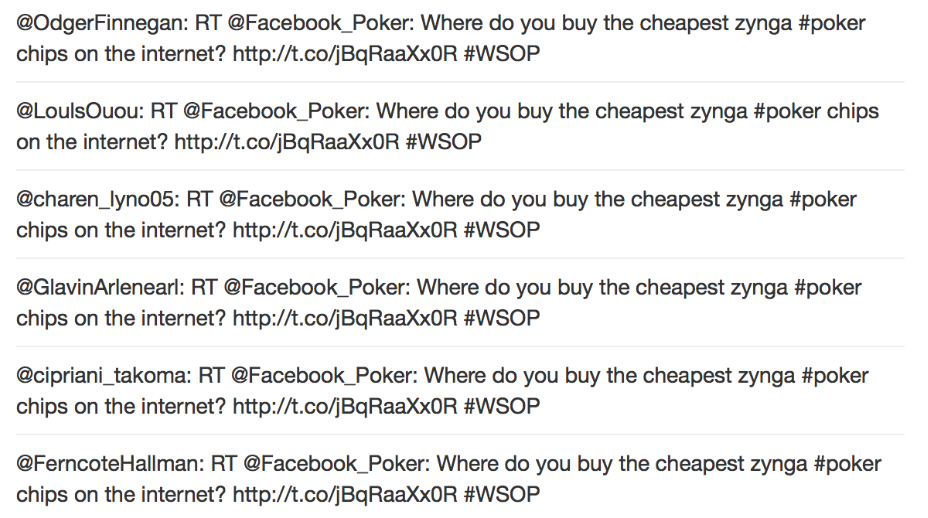
\includegraphics[width=\textwidth,height=\textheight,keepaspectratio]{src/img/bots.png}
\caption{Automated messages sent by bots\label{overflow}}
\end{figure}
\newline
Due to the way the Twitter stream API works: it sends a percentage of all tweets currently being exchanged that match your query, we were able to make another interesting observation. A large number of Twitter topic clusters are formed from messages from bots. Twitter bots produce automatic messages usually with spam or promotional links. For the topics we tested on, mostly programming language topics, we noticed a large number of clusters related to job advertisements which turned out to be automated messages.
In the figure we extracted an example of bot messages that are using a popular hashtag (World Series of Poker) to advertise a game. This also provides some indication that relying completely on hashtags in order to generate topics and cluster messages is not always very efficient. Bots might use trending topics to their advantage: most Twitter clients offer limited discovery features and usually just show tweets that match a certain hashtag, by using the same one, spam such as this can end up in your message list.